%% Chapter 16 — Documentation & Portfolio Assembly
%% Course 247-519-VA, Vanier College
%% Project Planning & Prototyping

\chapter{Documentation \& Portfolio Assembly}
\label{ch16}

\paragraph{Where this fits.}
Chapter~15 completed the intellectual-property checklist --- the final artifact
produced by Stage~3 field work.
This chapter sits at the Gate~3 threshold and performs a different task: it
compiles every artifact produced since Concept into a single, coherent portfolio
package that a review committee can navigate, audit, and sign off.
No new design work happens here.
The work is assembly, reconciliation, and gap closure.

\paragraph{Learning Objectives.}
After completing this chapter you will be able to:
\begin{enumerate}
  \item Assemble a portfolio by mapping each required section to the stage
        artifact that produced it.
  \item Reconcile an as-built BOM against the design BOM and record every
        deviation as a documented decision.
  \item Compute traceability coverage and close gaps before Gate~3 submission.
\end{enumerate}

Every chapter in this textbook asked you to produce a deliverable and submit it
as a portfolio entry.
This chapter collects those entries.
If the artifacts exist, assembly takes an afternoon.
If they do not --- if specifications were written from memory the night before
the review --- the team is not assembling a portfolio; it is fabricating one.
The distinction matters to a reviewer, and it will matter to a regulator.

% ─────────────────────────────────────────────────────────────────────────────
\section{Three Documentation Principles}
\label{sec:ch16-principles}
% ─────────────────────────────────────────────────────────────────────────────

Three principles underlie every documentation practice introduced in this
course.

\textbf{Record decisions, not outcomes.}\index{documentation!record decisions}
An outcome tells the reader what happened.
A decision record tells the reader why an alternative was chosen, what evidence
supported it, and who was accountable.
A test report that says ``the sort latency met spec'' is an outcome.
A test report that says ``the sort latency was measured at 94\,ms against a
specification of $\leq$104\,ms using the procedure in Appendix~B; the margin is
attributed to the dual-core scheduling change documented in ECO-003'' is a
decision record.
Only the second version allows a future engineer --- or a Gate~3 reviewer --- to
reproduce the result or extend the design.

\textbf{Enable reproduction.}\index{documentation!reproducibility}
A portfolio entry that cannot be used to reproduce the result it describes is
incomplete.
Reproducibility requires: the exact part numbers used (not the ones originally
specified), the exact test procedure followed (not a paraphrase), and the exact
configuration of the firmware or software at the time of the test (a Git commit
hash, not ``the latest version'').

\textbf{Documentation debt compounds.}\index{documentation debt}
A design decision not recorded at Stage~2 generates a question at Stage~3.
That question requires someone to reconstruct the reasoning from memory, email
threads, or bench notes --- work that takes longer than the original record would
have, and produces a less reliable result.
If the reconstructed rationale is wrong, it generates a defect that propagates
into Stage~4 and beyond.
The interest rate on documentation debt is not linear: one missed record in
Stage~2 can produce three rework cycles in Stage~4.

\medskip
If any section of the Gate~3 portfolio must be written from memory at assembly
time, the process broke down earlier.
The correct response is to flag the section for remediation, document what is
known, and record that the original decision was not captured at the time it was
made.
Fabricating confidence is worse than acknowledging a gap.

% ─────────────────────────────────────────────────────────────────────────────
\section{Compiling, Not Writing}
\label{sec:ch16-compiling}
% ─────────────────────────────────────────────────────────────────────────────

The central insight of this chapter is that the Gate~3 portfolio is
\emph{compiled}, not written.
Every section has a source: a stage gate, a chapter deliverable, a test record,
a procurement document.
Figure~\ref{fig:ch16-doc-parallel} shows the Stage-Gate phases across the top
and the documentation artifacts each phase is expected to produce along the
bottom.

\begin{figure}[htbp]
  \centering
  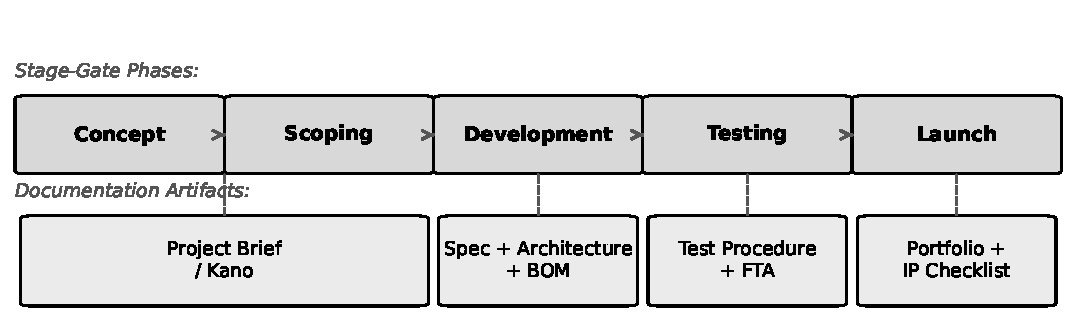
\includegraphics[width=0.88\textwidth]{images/fig_01_doc_parallel}
  \caption{Stage-Gate phases (top row) and the documentation artifacts
           each phase produces (bottom row).
           The portfolio is assembled from these artifacts at Gate~3;
           no section is written from scratch at assembly time.}
  \label{fig:ch16-doc-parallel}
\end{figure}

The key observation is temporal: the Project Brief and Kano analysis were
produced at Concept and Scoping; the specification, architecture, and BOM were
produced during Development; the test procedure and fault-tree analysis were
produced during Testing; the portfolio map and IP checklist were produced during
the Launch preparation.
A team that reaches Gate~3 without one of these artifacts is missing a stage
output, not a portfolio section.
The remedy is upstream, not cosmetic.

% ─────────────────────────────────────────────────────────────────────────────
\section{Portfolio Structure}
\label{sec:ch16-structure}
% ─────────────────────────────────────────────────────────────────────────────

The Gate~3 portfolio has fourteen sections.
Figure~\ref{fig:ch16-portfolio-map} maps each section to the chapter that
produced its source artifact.

\begin{figure}[htbp]
  \centering
  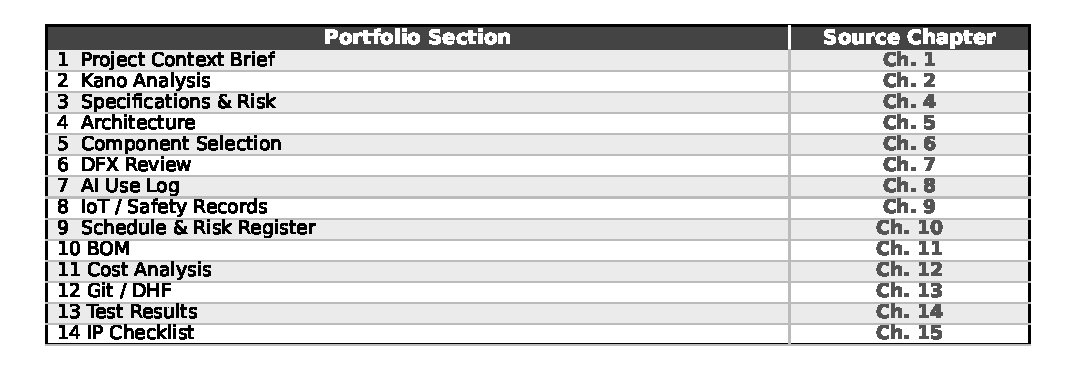
\includegraphics[width=0.88\textwidth]{images/fig_03_portfolio_map}
  \caption{Portfolio map: the fourteen required sections of the Gate~3
           documentation package and the source chapter that produced each
           artifact.
           Sections produced from memory rather than from documented stage
           outputs must be flagged for remediation.}
  \label{fig:ch16-portfolio-map}
\end{figure}

The fourteen sections form a logical narrative: who authorised the project and
why (Sections~1--2), what it must do and how it will do it (Sections~3--5),
what risks and quality requirements govern the design (Sections~6--8), how the
project was planned and controlled (Sections~9--10), what it costs and whether
the economics are viable (Sections~11--12), how the design was controlled and
what tests were run (Sections~12--13), and whether the design is free to
operate and market (Section~14).
A reviewer reads the portfolio in roughly this order; gaps in the narrative
signal gaps in the process.

Sections that appear thin --- a Kano analysis with no customer data, a risk
register with no updates since Stage~2, a BOM with no as-built reconciliation
--- do not become acceptable by being present.
Presence without substance fails a Gate~3 review as surely as absence.

% ─────────────────────────────────────────────────────────────────────────────
\section{The As-Built BOM}
\label{sec:ch16-as-built-bom}
% ─────────────────────────────────────────────────────────────────────────────

The \textbf{design BOM}\index{design BOM} records the parts the team intended
to use when the BOM was first approved.
The \textbf{as-built BOM}\index{as-built BOM} records the parts that were
actually used to build the prototype.
Both documents must appear in the Gate~3 package, and every line on which they
differ must carry a deviation record.

A \textbf{deviation record}\index{deviation record} contains four fields: the
original part (MPN, description, unit cost), the substituted part (MPN,
description, unit cost), the reason for substitution, and the disposition ---
either \emph{verified equivalent} (same electrical and mechanical performance
confirmed by datasheet comparison or test) or \emph{ECO issued} (an
Engineering Change Order was raised because the substitution changed a
functional parameter).

\paragraph{In Practice.}
A team building the IoT robotic sorting subsystem submitted a Gate~3 package
with a design BOM and an as-built BOM that were identical, despite the assembler
having substituted a motor driver during build because the original was out of
stock.
The reviewer discovered the substitution by inspecting the receipt; the package
was returned with a request for the deviation record, the datasheet comparison,
and the retest results on motor timing.
The team lost one week.
The deviation record would have taken twenty minutes to write at the time of
substitution.

\subsection{Worked Example --- Sorter As-Built Reconciliation}
\label{sec:ch16-asbuilt-worked}

The IoT robotic sorting subsystem design BOM had two line items that changed
between the design BOM and the as-built BOM:

\begin{enumerate}
  \item[(a)] \textbf{IMU:} Design BOM specified the MPU-6050 at \$12.40\,CAD.
        During procurement, the MPU-6050 was on a 14-week backorder.
        The ICM-42688-P was substituted at \$14.80\,CAD (+\$2.40 per unit).
        Disposition: \emph{verified equivalent} --- the ICM-42688-P is a
        drop-in replacement with a compatible I$^2$C register map at the
        addresses used by the firmware; verification performed by datasheet
        comparison and a 100-sample register-read test confirming identical
        output resolution and noise floor.

  \item[(b)] \textbf{PCB:} Design BOM specified a 2-layer board at \$32.00\,CAD.
        During testing, unacceptable EMC emissions were traced to signal-return
        path discontinuities on the 2-layer layout.
        A 4-layer board at \$41.00\,CAD (+\$9.00 per unit) was fabricated with
        dedicated power and ground planes.
        Disposition: \emph{ECO issued} --- ECO-007 documents the layer-count
        change, the EMC retest results (passed at $-6$\,dB margin), and the
        updated Gerber files committed to the Git design history file (DHF) at
        tag \texttt{v1.1-pcb-4layer}.
\end{enumerate}

The as-built unit cost increases by \$2.40 + \$9.00 = \$11.40 per unit relative
to the design BOM.
This figure must propagate to the cost analysis in Section~11 of the portfolio
and to the production cost projection in Chapter~17.

% ─────────────────────────────────────────────────────────────────────────────
\section{Traceability Coverage}
\label{sec:ch16-traceability}
% ─────────────────────────────────────────────────────────────────────────────

\subsection{The Traceability Matrix}
\label{sec:ch16-matrix}

A \textbf{traceability matrix}\index{traceability matrix} is a two-dimensional
grid that links every system requirement to at least one test case that verifies
it.
Rows represent requirements; columns represent test cases.
A filled cell means the test case exercises the requirement.
An empty cell means the requirement is either untested (a coverage gap) or that
the link has not yet been recorded (a documentation gap --- different in origin,
identical in risk).

The traceability matrix enforces a discipline that verbal assurances cannot:
it makes coverage visible, countable, and auditable.
A reviewer who asks ``how do you know R3 is met?'' expects a cell reference and
a test record, not a confident answer.

\subsection{Computing Coverage}
\label{sec:ch16-coverage-calc}

\textbf{Traceability coverage}\index{traceability coverage} is defined as the
fraction of required requirement-to-test links that are present in the matrix:

\begin{equation}\label{eq:ch16-coverage}
  \text{Coverage} = \frac{\text{number of requirements with at least one linked
  test case}}{\text{total number of requirements}} \times 100\,\%
\end{equation}

This definition counts at the requirement level: a requirement linked to three
test cases counts once in the numerator, the same as a requirement linked to
one.
The denominator is always the total count of requirements.
A Gate~3 submission should target 100\,\% coverage; any gap must either be
closed before submission or acknowledged with a written plan and timeline for
closure.

Note that the definition above measures whether each requirement has \emph{any}
link, not whether all intended links are present.
A more detailed audit counts the total number of planned requirement-to-test
pairs and computes the fraction of those pairs that are documented.
The worked example below uses the pair-counting approach because the sorter
design has a specific planned link that is missing.

\subsection{Worked Example --- Sorter Coverage Audit}
\label{sec:ch16-traceability-worked}

The IoT robotic sorting subsystem has four requirements and four test cases.
Figure~\ref{fig:ch16-traceability} shows the traceability matrix.

\begin{figure}[htbp]
  \centering
  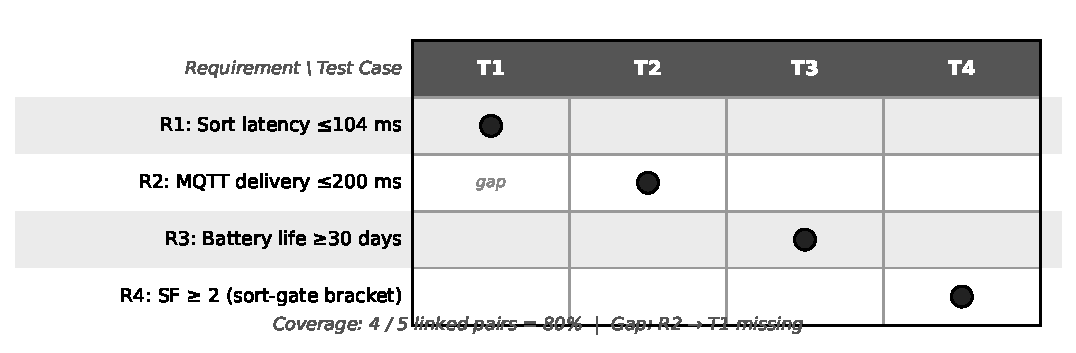
\includegraphics[width=0.88\textwidth]{images/fig_02_traceability}
  \caption{Traceability matrix for the IoT robotic sorting subsystem.
           Filled circles mark documented requirement-to-test links.
           The cell labelled ``gap'' (R2 $\to$ T1) identifies a planned link
           that is absent from the test record.
           Coverage: 4 of 5 planned pairs = 80\,\%.}
  \label{fig:ch16-traceability}
\end{figure}

The four requirements and their test links are:

\begin{enumerate}
  \item[(R1)] \textbf{Sort latency $\leq$ 104\,ms} --- linked to T1 (latency
        measurement test from Ch.~14, automated over 1\,000 sort cycles).
        Link documented. \checkmark

  \item[(R2)] \textbf{MQTT delivery $\leq$ 200\,ms} --- linked to T2
        (end-to-end message timing test, Ch.~14).
        Link documented. \checkmark\\
        R2 \emph{should also} link to T1, because the latency measurement test
        captures the sensor-to-publish pipeline including the MQTT stack.
        This link was planned during test design but is absent from the test
        record.
        \textbf{Gap identified.}

  \item[(R3)] \textbf{Battery life $\geq$ 30 days} --- linked to T3 (power
        budget verification using the calculation method from Ch.~9).
        Link documented. \checkmark

  \item[(R4)] \textbf{Safety factor SF $\geq$ 2 for sort-gate bracket} ---
        linked to T4 (static load test on bracket assembly).
        Link documented. \checkmark
\end{enumerate}

Of the 5 planned requirement-to-test pairs, 4 are present.
Applying Equation~\ref{eq:ch16-coverage}:

\begin{equation*}
  \text{Coverage} = \frac{4}{5} \times 100\,\% = 80\,\%
\end{equation*}

The gap is closed by adding the R2 $\to$ T1 link to the test record and
confirming that the latency test procedure includes the MQTT publish step in its
timing window.
If the current T1 procedure times only the mechanical sort and does not include
the MQTT publish, T1 must be extended --- a design-of-experiment change that
requires a new test run and an updated test report before Gate~3 submission.
After the link is added and confirmed, coverage rises to 5/5 = 100\,\%.

\paragraph{In Practice.}
A student team submitted a Gate~3 package for a temperature-controlled
enclosure with a traceability matrix showing 60\,\% coverage (3 of 5
requirements linked to tests).
The two unlinked requirements were control-loop stability and fan noise.
The review committee returned the package with a single action item: run the
missing tests and resubmit.
The team had assumed the reviewer would accept a verbal description of observed
behaviour in lieu of a test record.
The reviewer did not.
The retest took three days; writing the test procedures before the build would
have taken two hours.

\paragraph{Common Pitfalls.}
\begin{enumerate}
  \item[(a)] \textbf{Writing requirements from memory at Gate~3.}
        Requirements not captured in the specification document (Ch.~4) cannot
        be traced to tests without fabricating the traceability --- which a
        reviewer will detect by checking whether the test procedure predates the
        requirement.

  \item[(b)] \textbf{As-built BOM never reconciled.}
        Assemblers routinely substitute parts during build; if no one captures
        the substitution, the design BOM and the as-built BOM diverge silently.
        The divergence is discovered at the worst possible time --- during a
        production ramp or a regulatory audit.

  \item[(c)] \textbf{Assuming 100\,\% coverage without checking.}
        Coverage must be computed from the matrix, not asserted.
        A team that has run four tests for four requirements may still have
        80\,\% coverage if a planned link was never recorded.
        Count the cells.
\end{enumerate}

% ─────────────────────────────────────────────────────────────────────────────
\section*{Try It Yourself}
\addcontentsline{toc}{section}{Try It Yourself}
\label{sec:ch16-try}
% ─────────────────────────────────────────────────────────────────────────────

A 3-axis force sensor subsystem has three requirements: (R1) full-scale range
$\geq 50$\,N, (R2) linearity error $\leq 1$\,\%, (R3) drift $\leq 0.1$\,\%/\textdegree C.
Three test cases have been run: T1 (static load calibration), T2 (linearity
sweep), T3 (temperature cycling).
The current coverage matrix shows: R1 $\to$ T1 \checkmark, R2 $\to$ T2
\checkmark, R3 is not linked to any test case.

\begin{enumerate}
  \item[(a)] Compute the traceability coverage percentage using
        Equation~\ref{eq:ch16-coverage}.
        (Use the requirement-level definition: count requirements that have
        at least one link.)

  \item[(b)] Identify the coverage gap.
        Propose a specific test procedure --- including what stimulus is applied,
        what is measured, and what pass criterion is used --- that would close
        the gap and allow R3 $\to$ T3 to be documented as a verified link.

  \item[(c)] After the build, two BOM line items changed: the strain gauge
        changed from SG-A at \$3.20 to SG-B at \$4.80 (reason: mechanical fit
        incompatibility with the sensor housing); the signal amplifier changed
        from INA333 at \$2.10 to AD8221 at \$5.40 (reason: noise floor of
        INA333 exceeded the 1\,\% linearity budget under the supply voltage
        used).
        Compute the total BOM cost increase per unit (one of each component)
        and classify each substitution as: (i) record only, (ii) record and
        verify equivalence, or (iii) record and issue an ECO.
        Justify your classification.
\end{enumerate}

% ─────────────────────────────────────────────────────────────────────────────
\section*{Review Questions}
\addcontentsline{toc}{section}{Review Questions}
\label{sec:ch16-review}
% ─────────────────────────────────────────────────────────────────────────────

\begin{enumerate}
  \item \textbf{(Conceptual)} Explain the statement ``documentation debt
        compounds.''
        Give a concrete example of how failing to record a design decision
        in Stage~3 causes rework in Stage~4.

  \item \textbf{(Conceptual)} What is the difference between a design BOM and
        an as-built BOM?
        Why must both appear in the Gate~3 package?

  \item \textbf{(Applied, calculation)} A design has 6 requirements.
        The traceability matrix shows: R1 $\to$ T1, R2 $\to$ T2, R3 $\to$ T2,
        R4 $\to$ T3, R5 (no test linked), R6 $\to$ T4.
        Compute traceability coverage using Equation~\ref{eq:ch16-coverage}.
        What single action closes the gap?

  \item \textbf{(Applied)} An as-built BOM shows three substitutions:
        \begin{enumerate}
          \item[(a)] A resistor changed value (same footprint, \$0.05
                difference).
          \item[(b)] An MCU replaced with a pin-compatible alternative
                (\$3.20 more per unit).
          \item[(c)] A connector replaced with a non-standard alternative
                requiring a PCB spin.
        \end{enumerate}
        Classify each substitution as: (i) record only, (ii) record and verify
        equivalence, or (iii) record and issue an ECO.
        Justify your classification.

  \item \textbf{(Applied, multi-step)} A 5-requirement design has the
        following coverage matrix: R1 $\to$ T1, R2 $\to$ T1 and T2, R3
        $\to$ T3, R4 (no test linked), R5 $\to$ T2.
        \begin{enumerate}
          \item[(a)] Compute traceability coverage using
                Equation~\ref{eq:ch16-coverage}.
          \item[(b)] A new test T4 is added, linking to R4 and R5.
                Recompute coverage.
          \item[(c)] What percentage-point improvement does T4 add?
        \end{enumerate}
\end{enumerate}

% ─────────────────────────────────────────────────────────────────────────────
\section*{Portfolio Entry}
\addcontentsline{toc}{section}{Portfolio Entry}
\label{sec:ch16-artifact}
% ─────────────────────────────────────────────────────────────────────────────

Submit the following as your Gate~3 documentation package:

\begin{enumerate}
  \item[(a)] \textit{Assembled portfolio} --- all 14 sections listed in
        Figure~\ref{fig:ch16-portfolio-map} populated with artifacts from their
        source chapters.
        Sections produced from memory rather than from documented stage outputs
        must be flagged for remediation.

  \item[(b)] \textit{As-built BOM} --- reconciled against the design BOM with
        every deviation documented as a decision record (original part number,
        substituted part number, reason for change, and verified-equivalent or
        ECO reference).

  \item[(c)] \textit{Traceability matrix} --- all requirements listed, all
        test cases linked, coverage percentage computed using
        Equation~\ref{eq:ch16-coverage}.
        Any gap must be closed or explicitly acknowledged with a plan to close
        it before Gate~3 sign-off.
\end{enumerate}

This is the near-final version of your prototype documentation package.
Chapter~17 adds the production cost projection and the Gate~3 readiness
statement to complete it.

% ─────────────────────────────────────────────────────────────────────────────
\section*{Chapter Summary}
\addcontentsline{toc}{section}{Chapter Summary}
\label{sec:ch16-summary}
% ─────────────────────────────────────────────────────────────────────────────

The Gate~3 portfolio is compiled from artifacts produced at each Stage-Gate
phase, not written from memory at submission time.
Three principles govern documentation practice: record decisions not outcomes,
enable reproduction, and recognise that documentation debt compounds.
The fourteen-section portfolio map (Figure~\ref{fig:ch16-portfolio-map})
identifies the source chapter for every required section; any section that
cannot be traced to a stage artifact signals a process breakdown, not a writing
task.

The as-built BOM must be reconciled against the design BOM line by line.
Every deviation is a documented decision record --- part numbers, cost
difference, reason, and disposition (verified equivalent or ECO issued).
The sorter example showed two substitutions totalling \$11.40 per unit, both
fully documented and propagated to the cost analysis.

Traceability coverage is computed from the matrix using
Equation~\ref{eq:ch16-coverage}.
The sorter audit found one missing link (R2 $\to$ T1) giving 80\,\% coverage,
and prescribed a specific corrective action before submission.
A Gate~3 submission must reach 100\,\% coverage or carry explicit
acknowledgement and a closure plan for every remaining gap.

You now have a complete documentation package.
Chapter~17 adds the production economics --- the unit-cost projection and
break-even analysis --- and the Gate~3 readiness statement that converts the
portfolio into a formal gate submission.
